% ch06-ml.tex -- Clustering and dimension reduction
\chapter{Clustering and dimension reduction}\label{ch:cluster}

No labels, no targets, no test-set referee --- welcome to unsupervised
learning, where every output is a \emph{claim}, not a score. Two tools
dominate: clustering, which asserts that rows fall into groups, and
dimension reduction, which asserts that $d$ coordinates can be compressed
into fewer with acceptable loss. Both are immensely useful and both answer
``did it work?'' with ``compared to what?'' This chapter implements
$k$-means and PCA from scratch, runs hierarchical clustering, t-SNE and
UMAP, and then does the part most tutorials skip: it interrogates the
answers. A clustering that separates random noise is worthless; a
projection that invents separation is worse. The through-line from
Chapter 3 survives intact --- there is always a baseline, and there is
always a way the number can lie.\index{unsupervised learning}

\section{Unsupervised $\neq$ evaluation-free}\label{sec:unsupeval}

With no $\mathbf{y}$, metrics come in two species. \emph{External}
criteria compare the clustering to ground truth when it exists
(adjusted Rand index, ARI\index{adjusted Rand index}). \emph{Internal}
criteria score the geometry itself --- the silhouette
coefficient\index{silhouette} measures each point's fit to its own
cluster vs its runner-up: $s(i) = (b - a)/\max(a,b)$, mean over all
points. Internal scores are the only game in real deployments --- and
they can be gamed by the data itself, as the noise trap below shows.
Treat them like Chapter 3's metrics: useful, with a named baseline.

\section{$k$-means: Lloyd's iterations}\label{sec:kmeans}

\index{k-means}$k$-means alternates two cheap moves until nothing
improves: assign each point to its nearest centroid, then re-centre each
cluster at its members' mean. The objective --- total squared distance to
the assigned centroid (inertia) --- never increases, so the loop
converges; to \emph{a} minimum, not \emph{the} minimum, which is why
initialisation (k-means++\index{k-means++} spreads starts cleverly) and
restarts matter.

\lstinputlisting[language=Python,caption={\texttt{code/ch06/kmeans\_scratch.py}: Lloyd's algorithm + k-means++ init on \texttt{iris}.},label={lst:kmeans}]{code/ch06/kmeans_scratch.py}

\lstinputlisting[numbers=none]{code/ch06/kmeans_scratch.out.txt}

\begin{figure}[ht]\centering
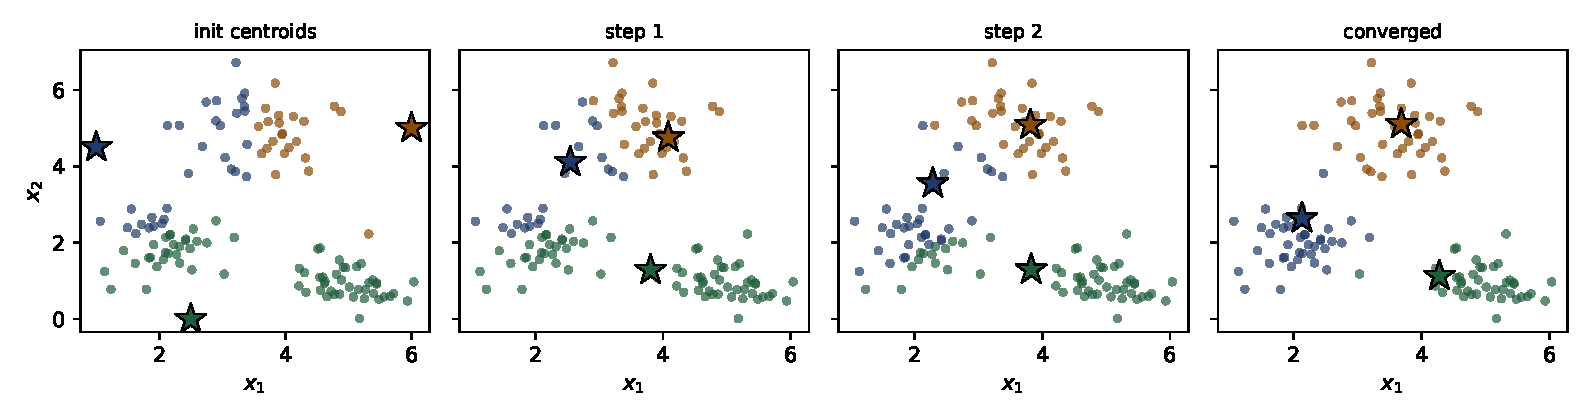
\includegraphics[width=\linewidth]{figures/ch06/lloyd_steps.pdf}
\caption{Lloyd's algorithm on 2-D synthetic data
(\texttt{figures/fig\_ch06\_lloyd\_steps.py}): assign, re-centre, repeat
--- centroids (stars) glide to the natural groups within a few
steps.}\label{fig:lloyd}
\end{figure}

\begin{example}[WE 6.1 --- The $k{=}2$ vs $k{=}3$ disagreement]\label{ex:kdisagree}
Strategy: let the silhouette argue with the truth and adjudicate.\par
\begin{solution}
On \texttt{iris}, silhouette peaks at $k{=}2$ ($0.681$) while ARI-vs-species
says $k{=}3$ is the better match ($0.730$ vs $0.540$): the internal
criterion prefers merging two species that overlap heavily, the external
criterion prefers the biology. Both are ``right'' about different questions
--- silhouette asks which partition is \emph{geometrically} cleanest, ARI
asks which matches a hidden label. The honest summary: iris has 3 species
and 2 clear clusters; report both numbers and let the claim carry the
caveat. (And k-means's own fragility shows in the seed sweep: seed 0
stalls at inertia $142.8$ vs the real minimum $78.9$ --- one bad start,
$80\%$ wasted.)\index{inertia}
\end{solution}
\end{example}

\section{Hierarchical clustering and linkage}\label{sec:hier}

\index{hierarchical clustering}Agglomerative clustering starts every point
as its own cluster and merges the cheapest pair until one cluster remains
--- the full history draws as a dendrogram\index{dendrogram}. The merge
rule (linkage) is the personality: \emph{single} takes nearest-neighbour
distance (chains straggly blobs together), \emph{complete} takes farthest
(tight, easily split groups), \emph{average} compromises, \emph{ward}
minimises added within-cluster variance (compact globes, the usual
default). Cutting the dendrogram at a height gives the clustering ---
Figure~\ref{fig:dendro} shows ward's clean 3-level structure on
\texttt{wine} vs single's unhelpful chain.

\begin{figure}[ht]\centering
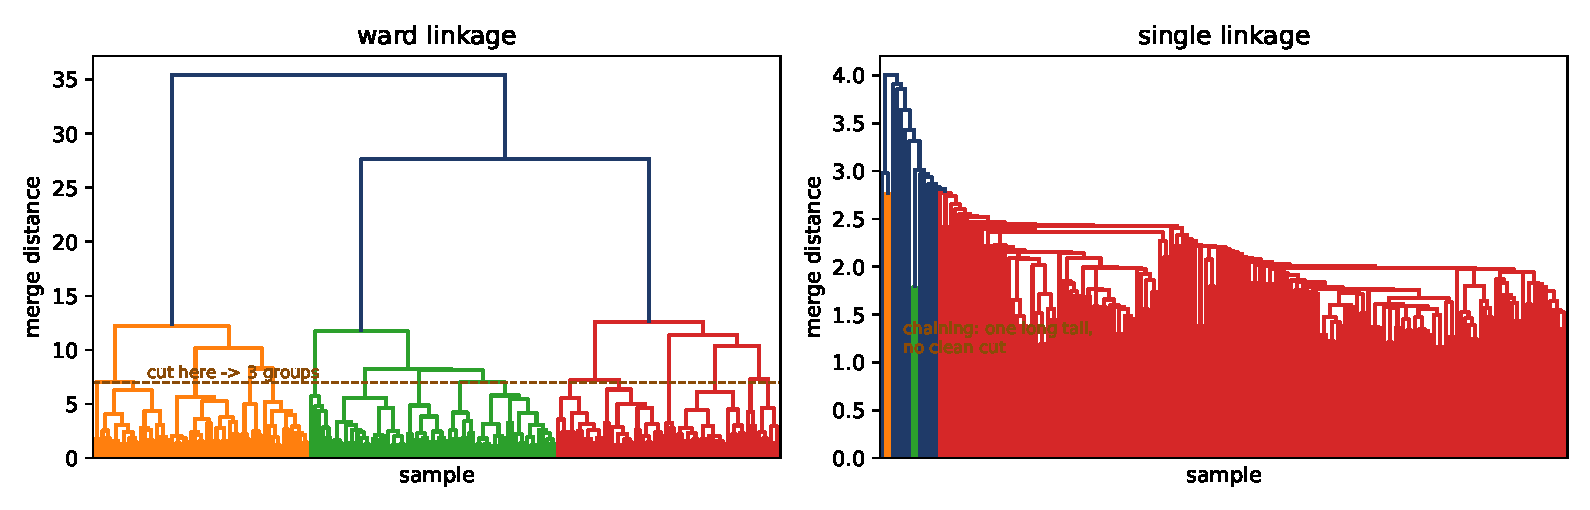
\includegraphics[width=\linewidth]{figures/ch06/dendro.pdf}
\caption{Ward vs single linkage on \texttt{wine}
(\texttt{figures/fig\_ch06\_dendro.py}): same data, two stories --- ward
offers an obvious 3-group cut; single linkage chains everything into one
tail. Choose linkage by the shape you are hunting.}\label{fig:dendro}
\end{figure}

\section{PCA via SVD: keep the variance, drop the dims}\label{sec:pca}

\index{PCA}\index{SVD}Principal component analysis finds the orthogonal
directions of maximum variance and projects onto the top $k$. Via the SVD
$X_c = USV^T$ of the centred matrix, components are columns of $V$,
variances are $S^2/(n{-}1)$, and reconstruction is
$\hat X = \mu + X_c V_k^T V_k$ --- the best rank-$k$ approximation in
squared error, provably.

\lstinputlisting[language=Python,caption={\texttt{code/ch06/pca\_svd.py}: PCA from the SVD on \texttt{digits}: variance kept per component, plus reconstruction error of one digit at $k\in\{10,30,60\}$.},label={lst:pca}]{code/ch06/pca_svd.py}

\lstinputlisting[numbers=none]{code/ch06/pca_svd.out.txt}

\begin{figure}[ht]\centering
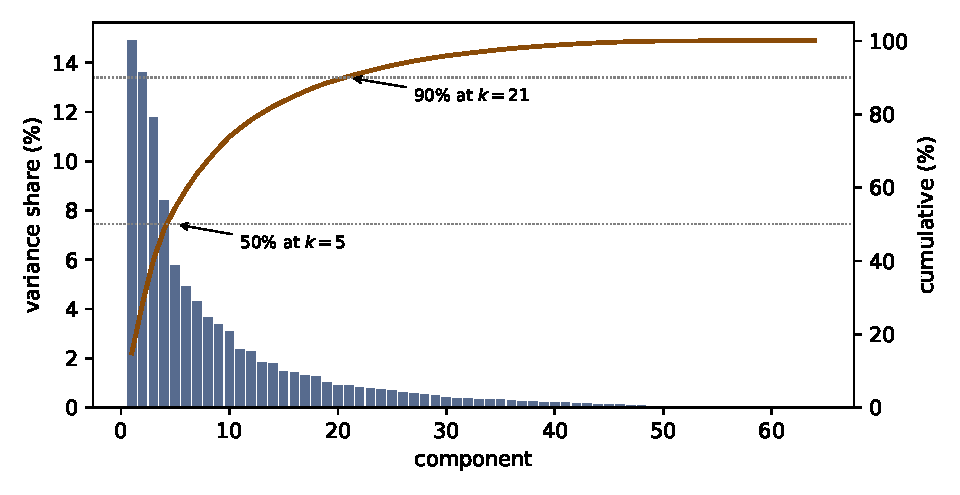
\includegraphics[width=0.7\linewidth]{figures/ch06/scree.pdf}
\caption{Scree and cumulative-variance curves on \texttt{digits}
(\texttt{figures/fig\_ch06\_scree.pdf}). Five components hold half the
variance; 21 hold $90\%$; the elbow is a budget question --- how much
reconstruction can the downstream task afford?}\label{fig:scree}
\end{figure}

\begin{example}[WE 6.2 --- The elbow is a budget]\label{ex:elbow}
Strategy: pick $k$ by what reconstruction error you can pay, not by a
ritual.\par
\begin{solution}
On \texttt{digits}: $k{=}5$ halves the variance, $k{=}13$ holds $80\%$,
$k{=}21$ holds $90\%$ --- and rebuilding one `8' from the top components
costs $7.9\%$ squared-error share at $k{=}10$, $0.9\%$ at $k{=}30$,
essentially nothing at $k{=}60$. The elbow ($\sim$k 5--10) is where cheap
variance ends; whether you stop there depends on whether the task is
visualisation ($k{=}2$), compression ($k{=}21$+), or denoising input to a
learner. PCA is a dial, not a destination.\index{reconstruction error}
\end{solution}
\end{example}

\begin{figure}[ht]\centering
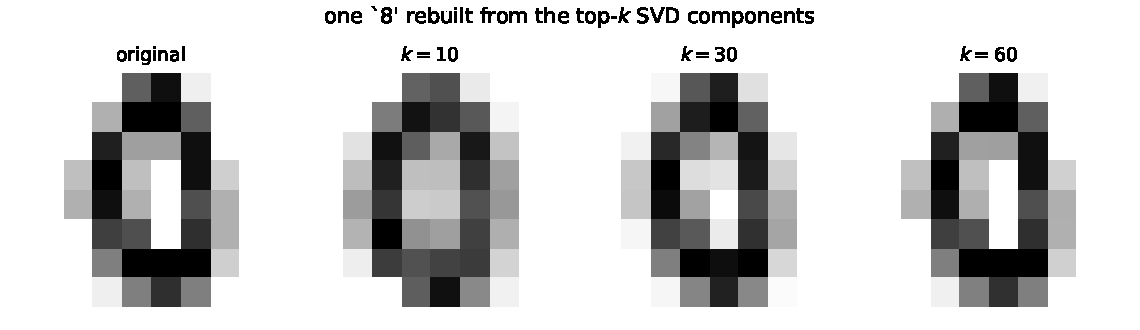
\includegraphics[width=0.9\linewidth]{figures/ch06/recon_strip.pdf}
\caption{WE 6.2 made visible (\texttt{figures/fig\_ch06\_recon\_strip.py}):
one digit rebuilt from the top-$k$ SVD components --- recognisable at
$k{=}10$, faithful at $k{=}60$.}\label{fig:recon}
\end{figure}

\section{Beyond linear: t-SNE and UMAP}\label{sec:tsne}

\index{t-SNE}\index{UMAP}Nonlinear embeddings optimise a different thing:
keep \emph{neighbours} close at any cost to global shape. t-SNE minimises
the KL divergence between high-$d$ and low-$d$ neighbourhood
distributions; UMAP models the data's fuzzy graph and embeds it. Both
produce gorgeous local clusters --- and both can fabricate separation
that isn't in the data, or hide separation that is. Sizes, distances, and
cluster counts in their output are \emph{not} quantitative.

\begin{figure}[ht]\centering
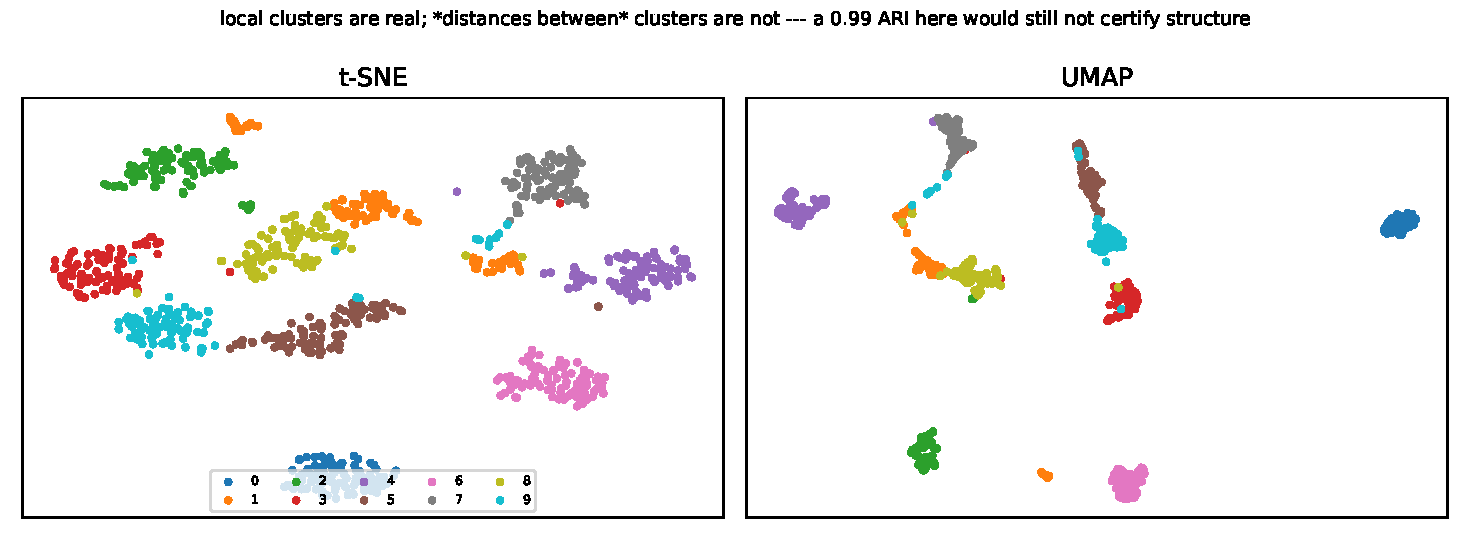
\includegraphics[width=\linewidth]{figures/ch06/tsne_umap.pdf}
\caption{t-SNE vs UMAP on \texttt{digits}
(\texttt{figures/fig\_ch06\_tsne\_umap.py}): local clusters mostly real,
global distances not. A big empty gap on the plot may be an artefact of
the optimiser, not the data --- verify with labels or a supervised
metric.}\label{fig:tsne}
\end{figure}

\section{Scaling first: the silent failure}\label{sec:scalefirst}

Clustering is distance, and distance is units. On raw \texttt{wine},
\texttt{proline}'s range (300--1700) makes \texttt{alcohol}'s (11--15)
irrelevant: the ``clusters'' found are unit artefacts. Standardise first
--- the same two features then yield meaningful groups
(Figure~\ref{fig:scaling}).

\begin{figure}[ht]\centering
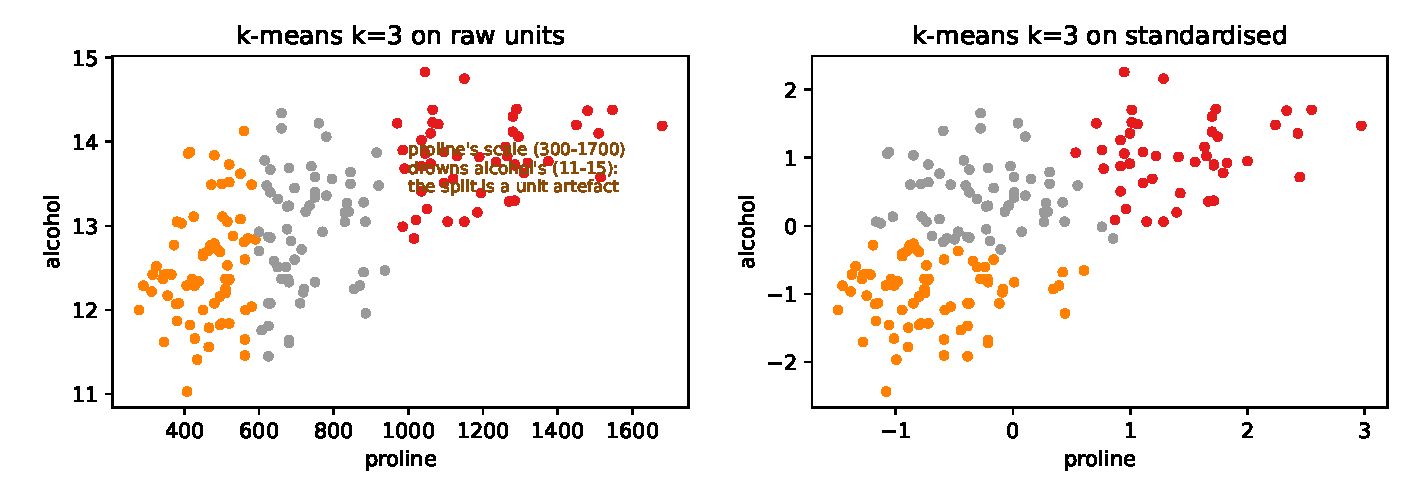
\includegraphics[width=\linewidth]{figures/ch06/scaling.pdf}
\caption{$k$-means on two wine features before/after standardising
(\texttt{figures/fig\_ch06\_scaling.py}): raw units let the
largest-magnitude column dictate every distance --- a Chapter 3 lesson
returned, unsupervised.}\label{fig:scaling}
\end{figure}

\section{The clusters-in-noise trap}\label{sec:trap}

\lstinputlisting[language=Python,caption={\texttt{code/ch06/cluster\_lib.py}: sklearn KMeans/Agglomerative on \texttt{digits}, the iris silhouette sweep, and k-means on pure uniform noise --- the trap this chapter exists to warn about.},label={lst:clusterlib}]{code/ch06/cluster_lib.py}

\lstinputlisting[numbers=none]{code/ch06/cluster_lib.out.txt}

\begin{example}[WE 6.3 --- Clusters that were never there]\label{ex:noise}
Strategy: run the pipeline on data where you \emph{know} there are no
clusters, and see what it reports.\par
\begin{solution}
Uniform random data, 300 points in 8 dims, and k-means dutifully returns
``clusters'' with silhouette $0.10$ --- small but nonzero, because any
partition of finite data has some shape. The real failure is
\emph{believing} the score without a null: rerun the same pipeline on a
null baseline (uniform, or shuffle each column) and compare silhouettes
--- real structure sits far above noise. Every clustering claim needs
this control the way every accuracy needs its lazy baseline.
\end{solution}
\end{example}

\begin{wins}
What you can now do: implement Lloyd's + k-means++; compute silhouette
and ARI and say what each measures; cut a dendrogram and choose a
linkage; do PCA by SVD and price components by variance; run t-SNE/UMAP
while knowing what they can't certify; catch the two silent failures ---
unscaled distances and noise-clustering --- with null baselines.
\end{wins}

\section{Common mistakes}

\begin{description}
\item[Clustering without scaling] The largest-unit column wins every
  distance --- standardise before anything that touches $\|x - x'\|$.
\item[Assuming $k$] Choosing $k$ by the silhouette of the k you wanted
  anyway is a self-fulfilling metric --- sweep, and show the curve.
\item[One seed, one answer] k-means is multi-modal; seed 0 cost $80\%$
  extra inertia in the listing --- \texttt{n\_init} exists for a reason.
\item[Treating silhouette as truth] It's a shape score, not a structure
  oracle --- noise clusters score nonzero too. Null-baseline first.
\item[Over-reading t-SNE] Cluster sizes, gaps, and counts in the
  embedding are aesthetic, not evidence --- verify with an external
  metric.
\item[Forgetting PCA centres] PCA on uncentred data finds the mean
  direction, not the variance direction --- centre always.
\item[Believing the dendrogram's $y$-axis at face value] Merge heights
  are in the linkage's units; comparing across linkages needs care.
\item[Reconstruction without a budget] Picking $k$ by the elbow shape
  rather than downstream tolerance --- the elbow is a budget question.
\item[Clustering the raw features when a projection is cleaner] On
  high-$d$ data, cluster in PCA space or with a method that respects
  density, not raw euclidean $d$-space.
\end{description}

\section{Summary table}

\begin{tabularx}{\linewidth}{@{}l l X@{}}
\toprule
\textbf{Tool} & \textbf{What it optimises} & \textbf{Watch out for}\\
\midrule
$k$-means & within-cluster squared dist.\ & init, $k$, globes only\\
Hierarchical & linkage merge cost & linkage = shape assumption\\
PCA & variance kept per component & centre first; linear only\\
t-SNE & local neighbourhood KL & distances aren't quantitative\\
UMAP & fuzzy graph embedding & same caveat, faster at scale\\
Silhouette & own-vs-runner-up fit & shape, not truth\\
ARI & match to external labels & needs labels you may not have\\
\bottomrule
\end{tabularx}

\section{Drill --- five concept questions}

\begin{enumerate}
\item Which two moves does Lloyd's algorithm alternate, and what
  quantity provably never increases?
\item A dendrogram cut at a higher level produces more or fewer
  clusters --- and what does the linkage control?
\item On \texttt{iris}, silhouette prefers $k{=}2$ and ARI prefers
  $k{=}3$. Which is ``correct,'' and what question does each answer?
\item Name two things a t-SNE plot cannot certify even when it looks
  beautiful.
\item Why does clustering \texttt{wine} on raw units effectively ignore
  the \texttt{alcohol} column?
\end{enumerate}

\section*{Further reading}
\begin{itemize}
\item Hastie, Tibshirani \& Friedman --- \emph{ESL}, ch.~14
  (unsupervised). \url{https://hastie.su.domains/ElemStatLearn/} ---
  k-means, hierarchical, and PCA in the reference register.
\item scikit-learn --- \emph{Clustering} user guide.
  \url{https://scikit-learn.org/stable/modules/clustering.html} ---
  KMeans, Agglomerative, DBSCAN and the metrics used here.
\item scikit-learn --- \emph{Decomposition} user guide.
  \url{https://scikit-learn.org/stable/modules/decomposition.html} ---
  PCA (and variants) behind Listing~\ref{lst:pca}.
\item van der Maaten \& Hinton --- ``How to Use t-SNE Effectively,''
  \emph{Distill} (2016). \url{https://distill.pub/2016/misread-tsne/} ---
  the canonical ``what t-SNE can't tell you''; read before publishing
  any t-SNE figure.
\item UMAP documentation. \url{https://umap-learn.readthedocs.io/en/latest/}
  --- parameters that control local-vs-global preservation.
\item scikit-learn --- \texttt{silhouette\_score} reference.
  \url{https://scikit-learn.org/stable/modules/generated/sklearn.metrics.silhouette_score.html}
  --- the internal metric behind WE~6.1 and the trap.
\item SciPy --- \emph{Hierarchical clustering} reference.
  \url{https://docs.scipy.org/doc/scipy/reference/cluster.hierarchy.html}
  --- linkage rules and dendrogram API used in Figure~\ref{fig:dendro}.
\end{itemize}

\begin{rulebox}{Watch instead (if you'd rather see it)}
\begin{itemize}
\item \textbf{StatQuest: Principal Component Analysis (PCA),
  Step-by-Step} (21:57). StatQuest with Josh Starmer.
  \url{https://www.youtube.com/watch?v=FgakZw6K1QQ} --- SVD/variance
  walkthrough matching \S\ref{sec:pca}. Accessed 2026-10-11.
\item \textbf{StatQuest: t-SNE, Clearly Explained} (11:47). StatQuest
  with Josh Starmer. \url{https://www.youtube.com/watch?v=NEaUSP4YerM}
  --- perplexity and the embedding objective matching \S\ref{sec:tsne}.
  Accessed 2026-10-11.
\item \textbf{StatQuest: K-means clustering} (8:30). StatQuest with Josh
  Starmer. \url{https://www.youtube.com/watch?v=4b5d3muPQmA} --- Lloyd's
  iterations matching \S\ref{sec:kmeans}. Accessed 2026-10-11.
\end{itemize}
\end{rulebox}

\chapternotes
\begin{enumerate}
\item k-means++ init is Arthur \& Vassilvitskii (2007) --- the
  ``probabilistic spread'' the scratch listing implements.
\item Ward linkage's merge cost is the within-cluster variance delta ---
  the reason its dendrograms look like balanced trees.
\item PCA $\leftrightarrow$ SVD is exact: components are right-singular
  vectors; the ``eigendecomposition of the covariance'' formulation is
  the same computation through the covariance's own SVD.
\item DBSCAN and density methods cover the non-convex cases k-means
  can't --- sklearn's clustering guide (Further reading) is the tour.
\item The silhouette-on-noise effect is why ``which $k$'' papers exist
  --- null-baseline comparison is the practical control every time.
\end{enumerate}

\section*{Exercises}

\emph{[easy]}
\begin{exercise}
Compute the silhouette of a point with $a{=}1.0$, $b{=}3.0$ --- and say
what makes $s(i)$ negative.
\end{exercise}
\begin{exercise}
Which linkage produces chained clusters? Name the mechanism in one
sentence.
\end{exercise}
\begin{exercise}
From the scree data, how many \texttt{digits} components hold $80\%$ of
variance? $90\%$?
\end{exercise}

\emph{[medium]}
\begin{exercise}
Implement \texttt{silhouette(X, z)} with pairwise distances and verify
against sklearn on \texttt{iris} $k{=}3$.
\end{exercise}
\begin{exercise}
Re-run the iris $k$-sweep on \emph{standardised} data --- does
silhouette's $k{=}2$ preference survive? Explain with units.
\end{exercise}
\begin{exercise}
Reproduce Figure~\ref{fig:dendro} with \texttt{average} linkage added;
which cut best matches the 3 true wine classes (ARI)?
\end{exercise}
\begin{exercise}
Reconstruct \emph{every} digit at $k{=}21$ and compute the mean
squared-error share vs the scree's $90\%$ claim.
\end{exercise}
\begin{exercise}
Cluster \texttt{digits} projected to its top-30 PCs instead of raw 64-D;
report ARI and silhouette change.
\end{exercise}
\begin{exercise}
Re-run t-SNE at perplexity 5 and 50 on \texttt{digits}; describe which
panels of Figure~\ref{fig:tsne} change and what stays invariant.
\end{exercise}

\emph{[hard]}
\begin{exercise}
Derive PCA's objective: show maximising projected variance and
minimising reconstruction error give the same top-$k$ eigenvectors of
$X_c^TX_c$.
\end{exercise}
\begin{exercise}
Prove Lloyd's algorithm converges: inertia is non-increasing in both
steps and bounded below --- then explain why it can still hit a local
minimum (use the seed-0 case).
\end{exercise}
\begin{exercise}
Build a null-baseline protocol for ``does this dataset cluster at
all?'': specify the null, the statistic, and the decision rule ---
apply it to \texttt{wine}.
\end{exercise}
\begin{exercise}
Show t-SNE distances aren't quantitative: construct two 2-D point sets
whose inter-cluster gap on the embedding differs by 3$\times$ while the
data gap is identical.
\end{exercise}
\begin{exercise}
Prove k-means's objective is equivalent to within-cluster variance ---
i.e.\ minimising $\sum\|x - \mu_{c(x)}\|^2$ equals minimising the sum of
cluster variances.
\end{exercise}

\section*{Hints and answers}
\begin{description}
\item[6.1] $s = (3-1)/3 = 0.667$; $s<0$ when the runner-up is closer
  than home.
\item[6.2] Single linkage --- merging on the closest pair never lets
  outliers detach.
\item[6.3] $13$ and $21$ components.
\item[6.4] Mean over points of $(b-a)/\max(a,b)$; expect $\approx 0.55$.
\item[6.5] Same preference --- standardising reshuffles which feature
  dominates, not whether 2 vs 3 is geometrically cleaner.
\item[6.6] Ward usually beats average on ARI; the cut height decides
  the count.
\item[6.7] Mean error share should land near $1 - 0.90 = 0.10$.
\item[6.8] Usually improves ARI a little --- PCA drops noise dims that
  distance otherwise counts.
\item[6.9] Low perplexity fragments clusters; high merges them ---
  local membership persists, global layout shifts.
\item[6.10] Write both objectives, expand the residual into
  parallel/orthogonal parts, and read the eigenproblem.
\item[6.11] Both updates decrease or hold inertia and the space of
  assignments is finite --- but the fixed point is only locally
  optimal; seed 0 found a saddle of the objective.
\item[6.12] Permute each column independently to destroy joint
  structure; compare silhouette to its null distribution; decide by a
  gap statistic or a quantile.
\item[6.13] Two blobs at distances 5 and 8 embed with arbitrary-looking
  gaps --- the objective only preserves neighbours.
\item[6.14] Expand $\sum_{c}\sum_{x\in c}\|x-\mu_c\|^2$ and recognise
  each cluster's variance term; the assignments and means are the same
  optimisation.
\end{description}
